\begin{figure}
\centering
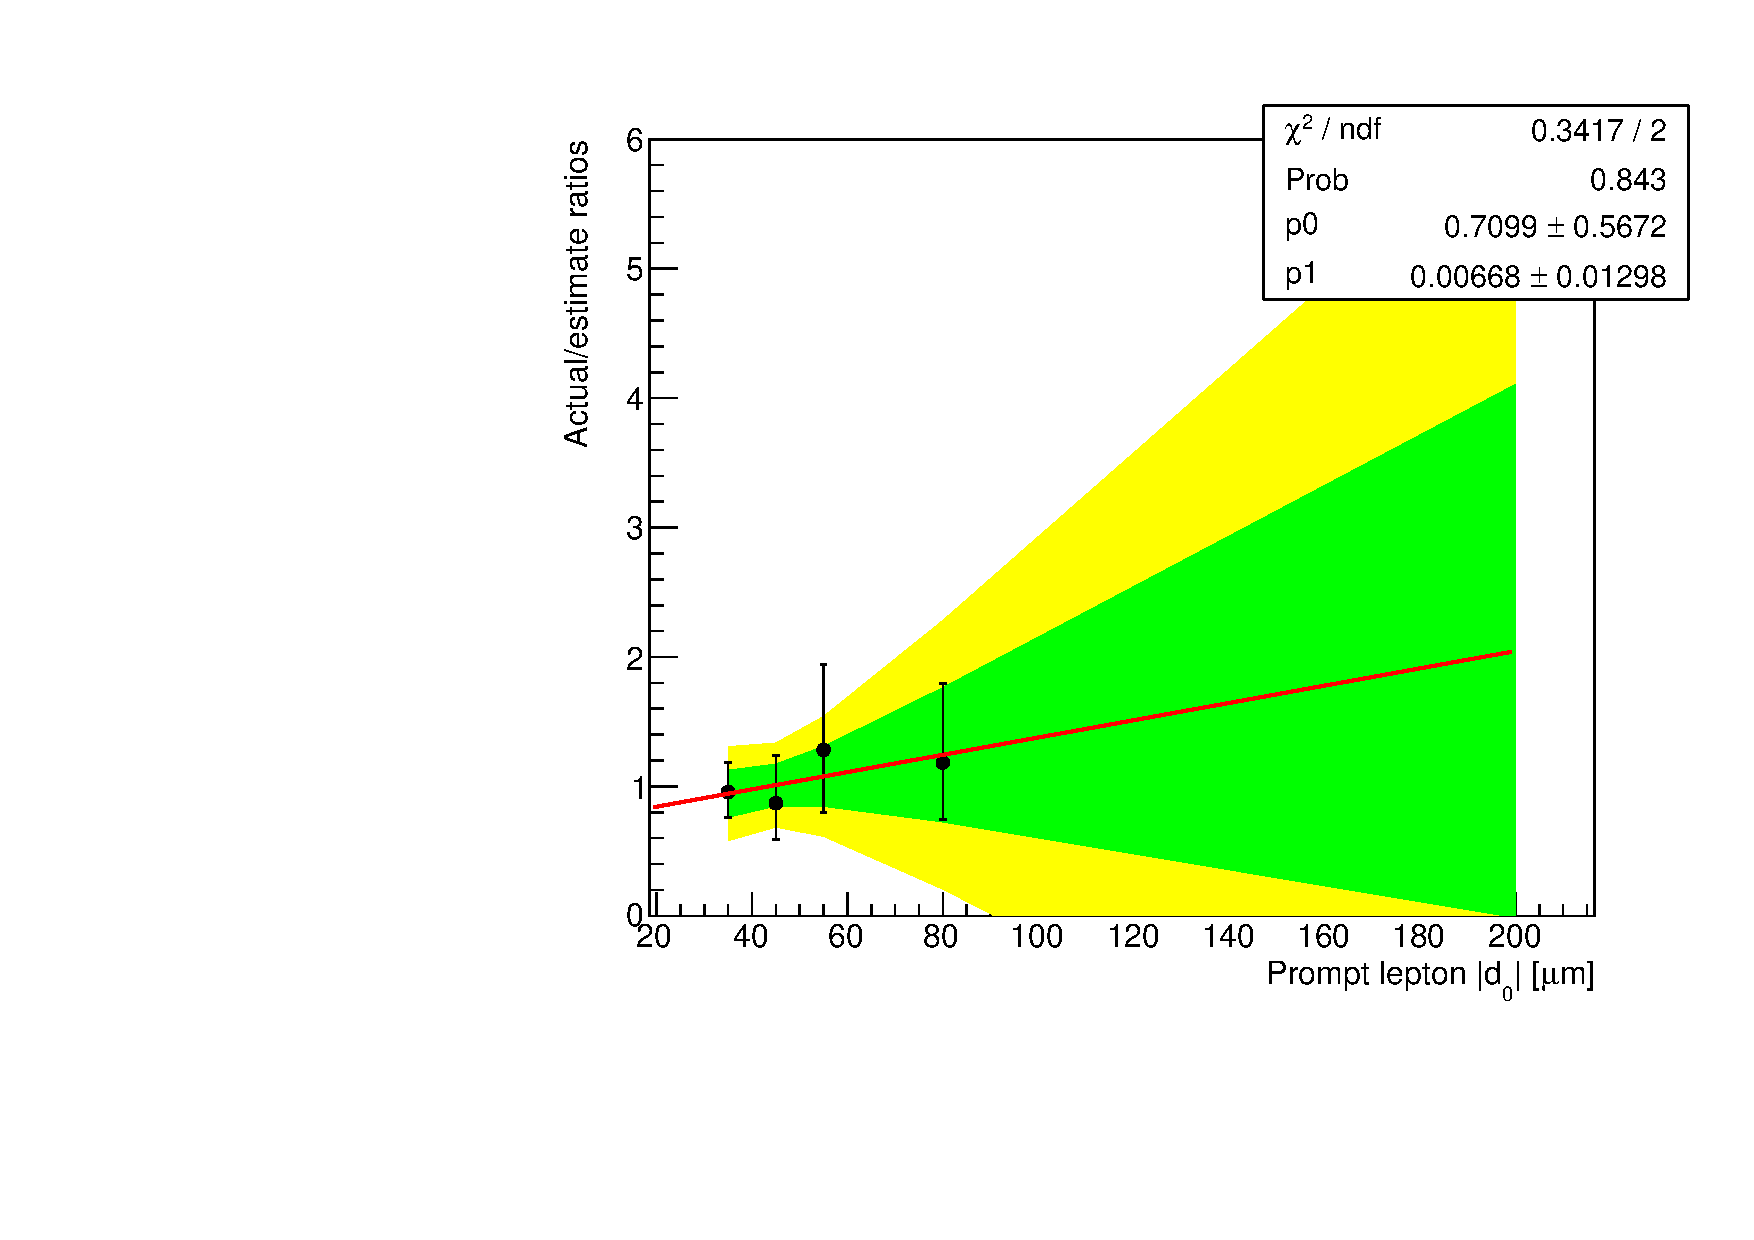
\includegraphics[width=0.45\textwidth]{figures/bg/emu_data_2016_displacedElectron_ratiosVsPromptD0.pdf}
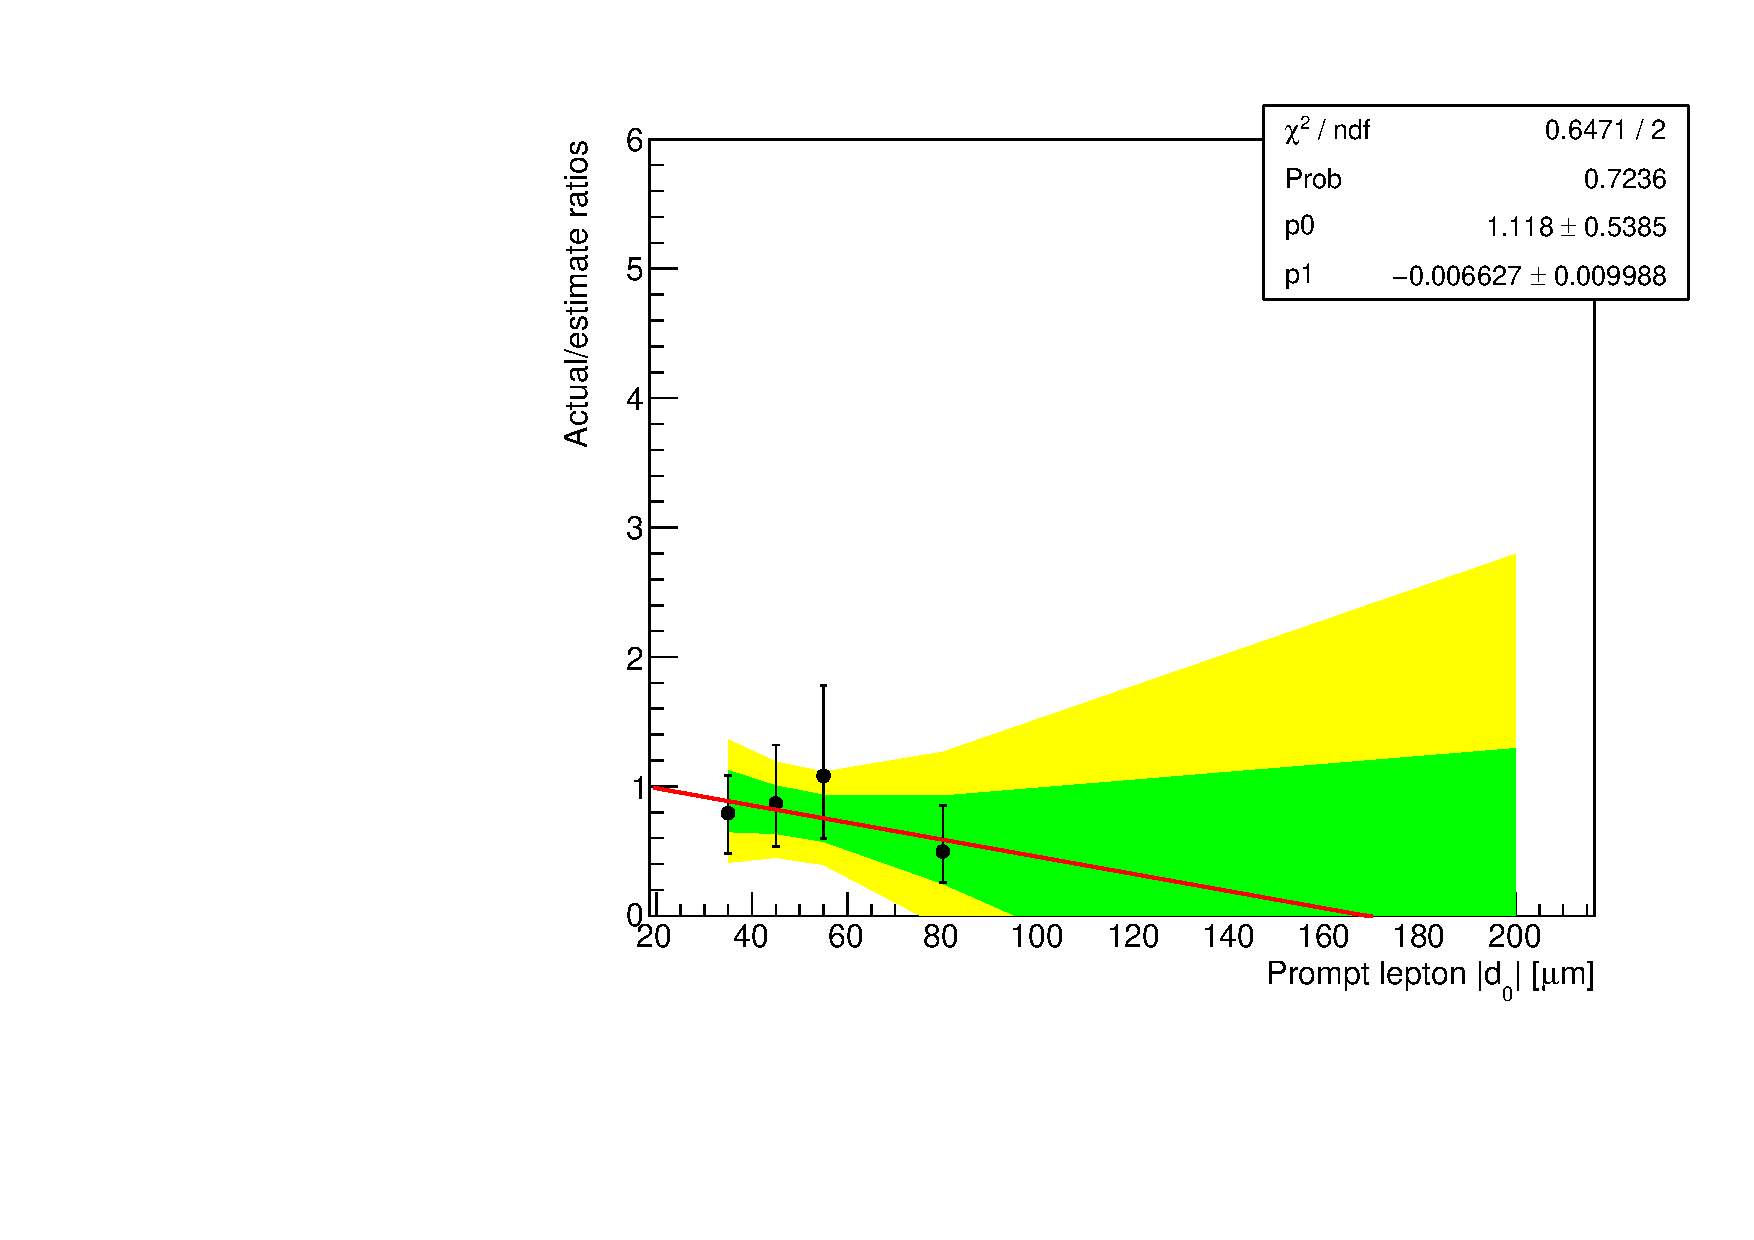
\includegraphics[width=0.45\textwidth]{figures/bg/emu_data_2016_displacedMuon_ratiosVsPromptD0.pdf}
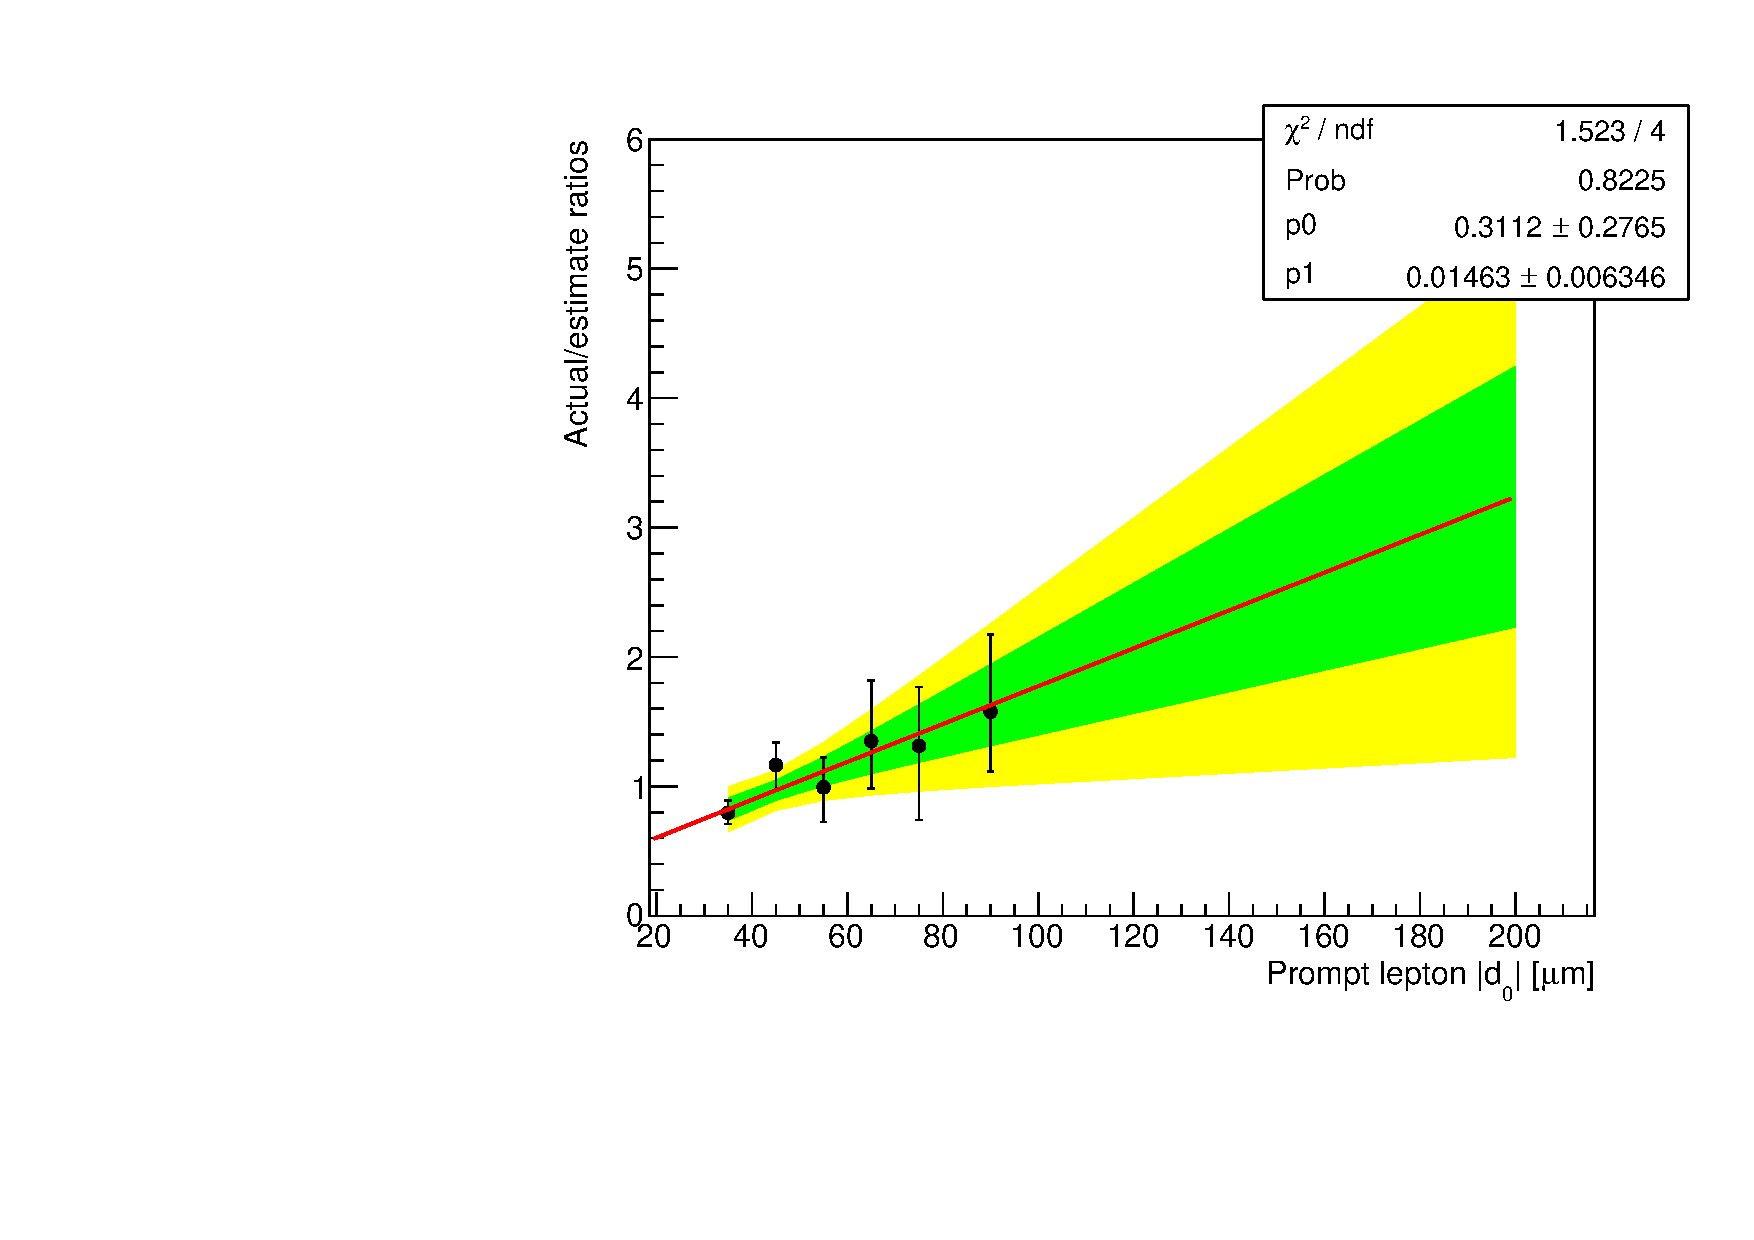
\includegraphics[width=0.45\textwidth]{figures/bg/emu_data_2017_2018_displacedElectron_ratiosVsPromptD0.pdf}
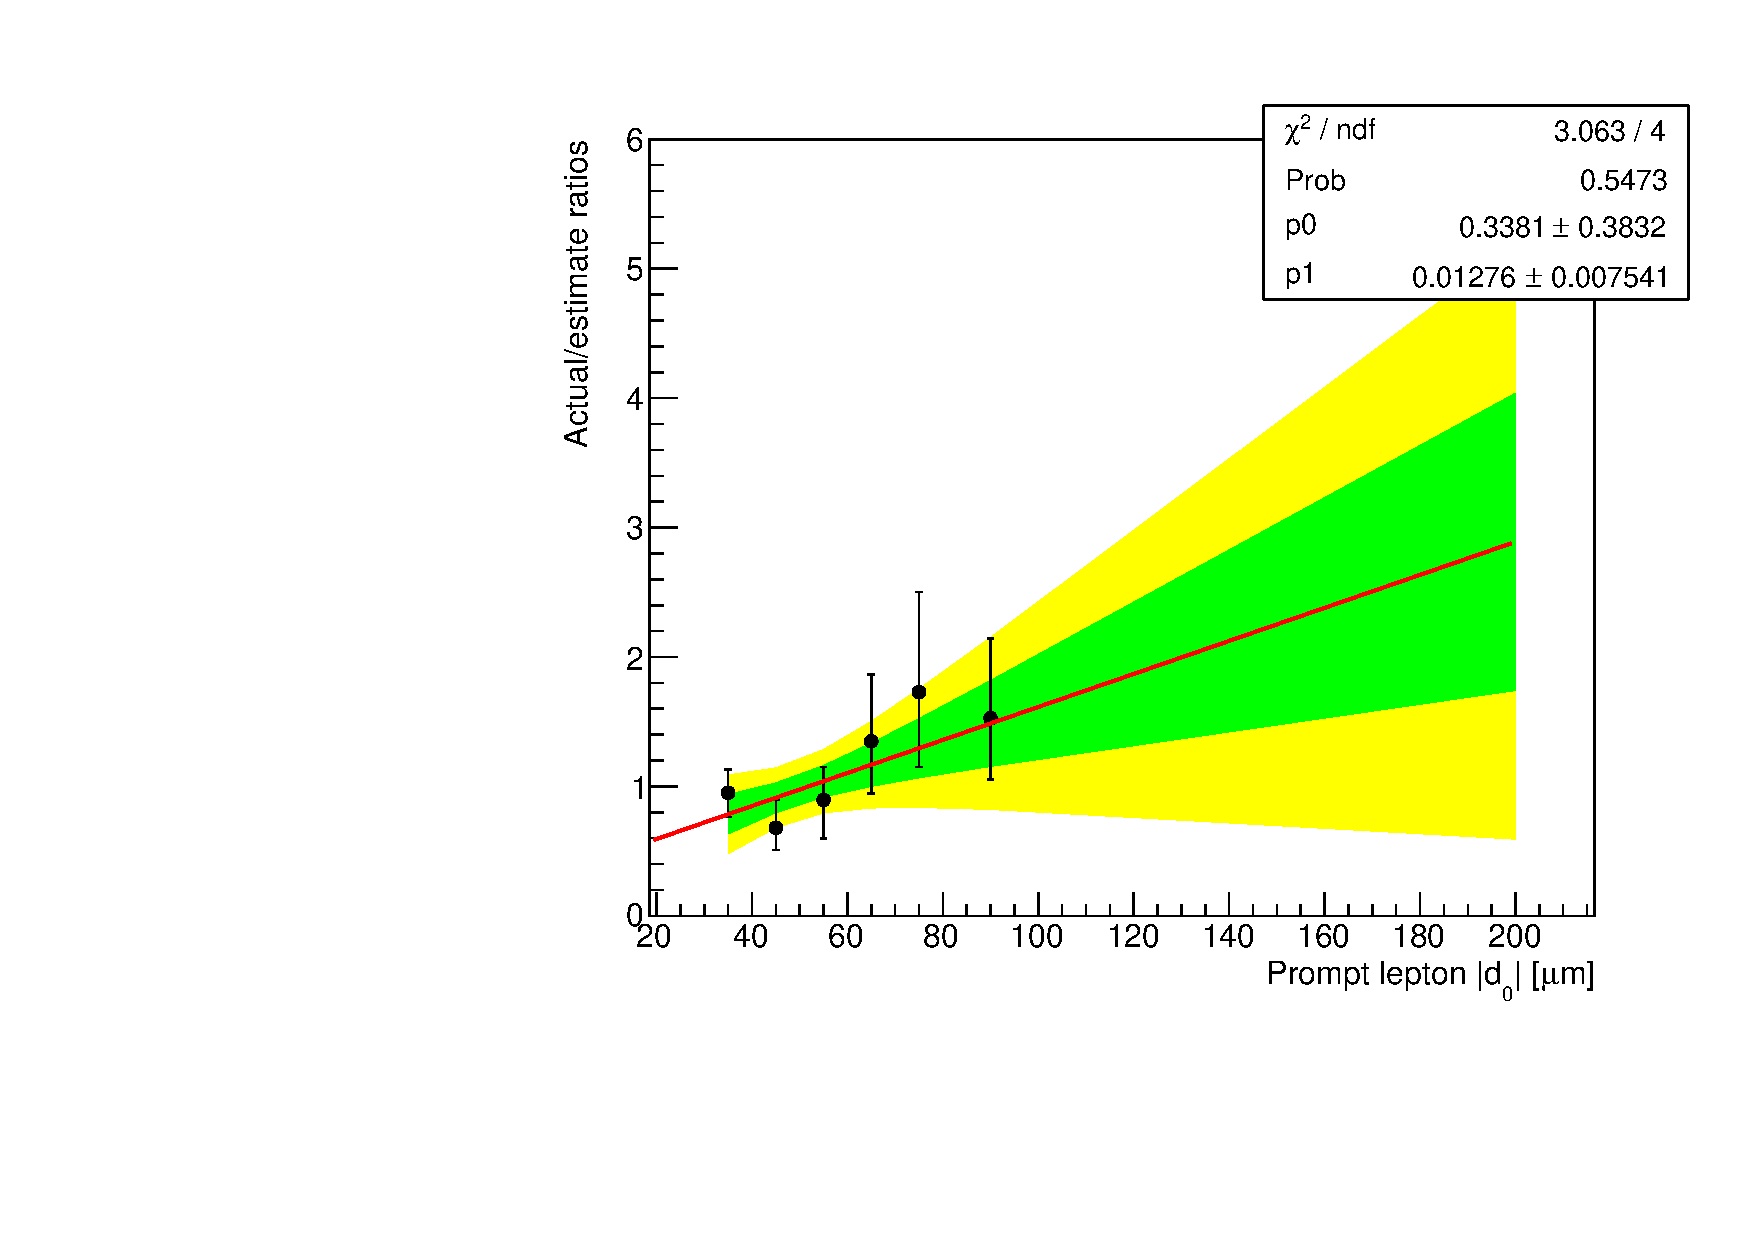
\includegraphics[width=0.45\textwidth]{figures/bg/emu_data_2017_2018_displacedMuon_ratiosVsPromptD0.pdf}
\caption{Background estimation closure tests in data, in 100--\SI{500}{\um} subregions of regions B (left) and C (right) in the $\Pe\Pgm$ channel. Each plot shows the ratio of the actual to the estimated number of events as a function of the prompt lepton \ad in 2016 (top) and 2017--18 (bottom). A linear fit is shown in black along with the \SI{68}{\percent} and \SI{95}{\percent} confidence intervals of the extrapolated fit value.}
\label{100to500um_fits_emu}
\end{figure}


\begin{figure}
\centering
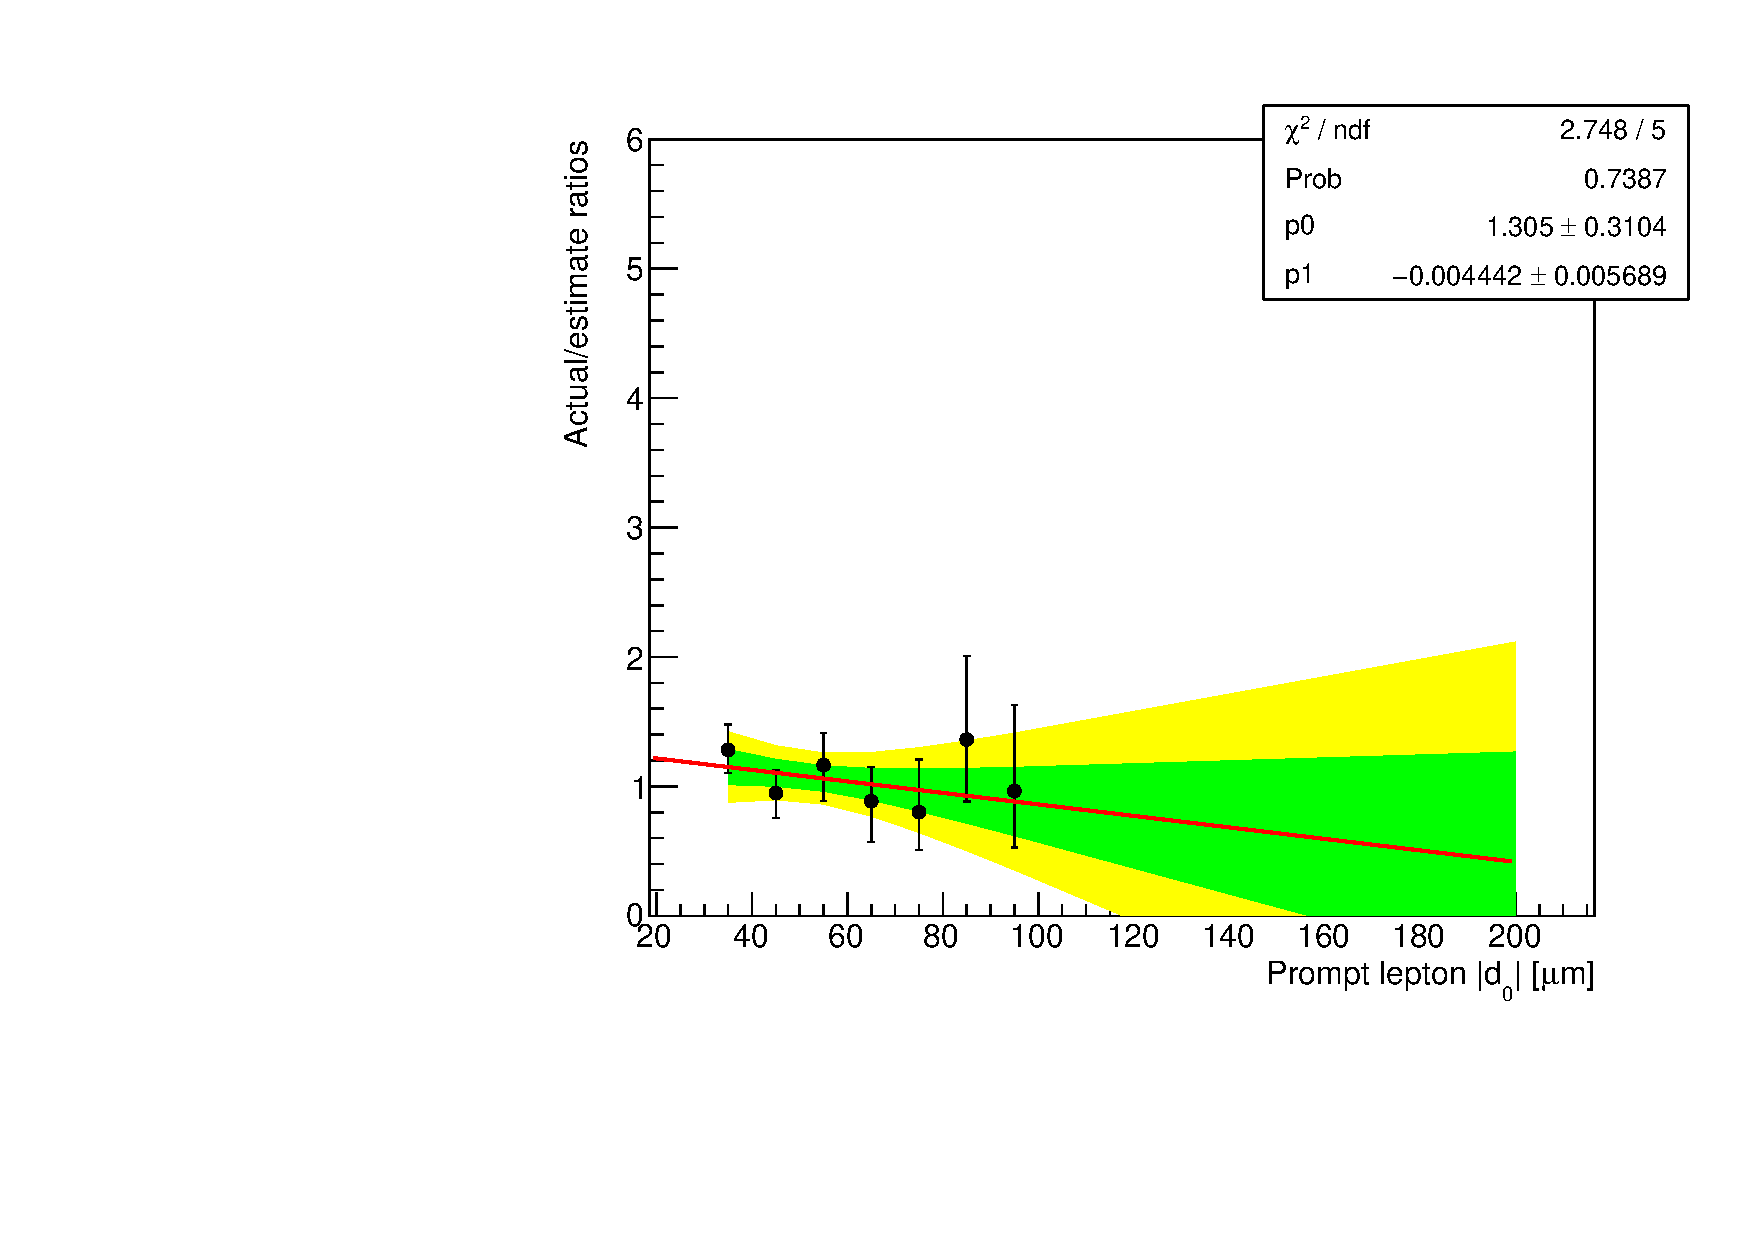
\includegraphics[width=0.45\textwidth]{figures/bg/ee_data_2016_displacedLeading_ratiosVsPromptD0.pdf}
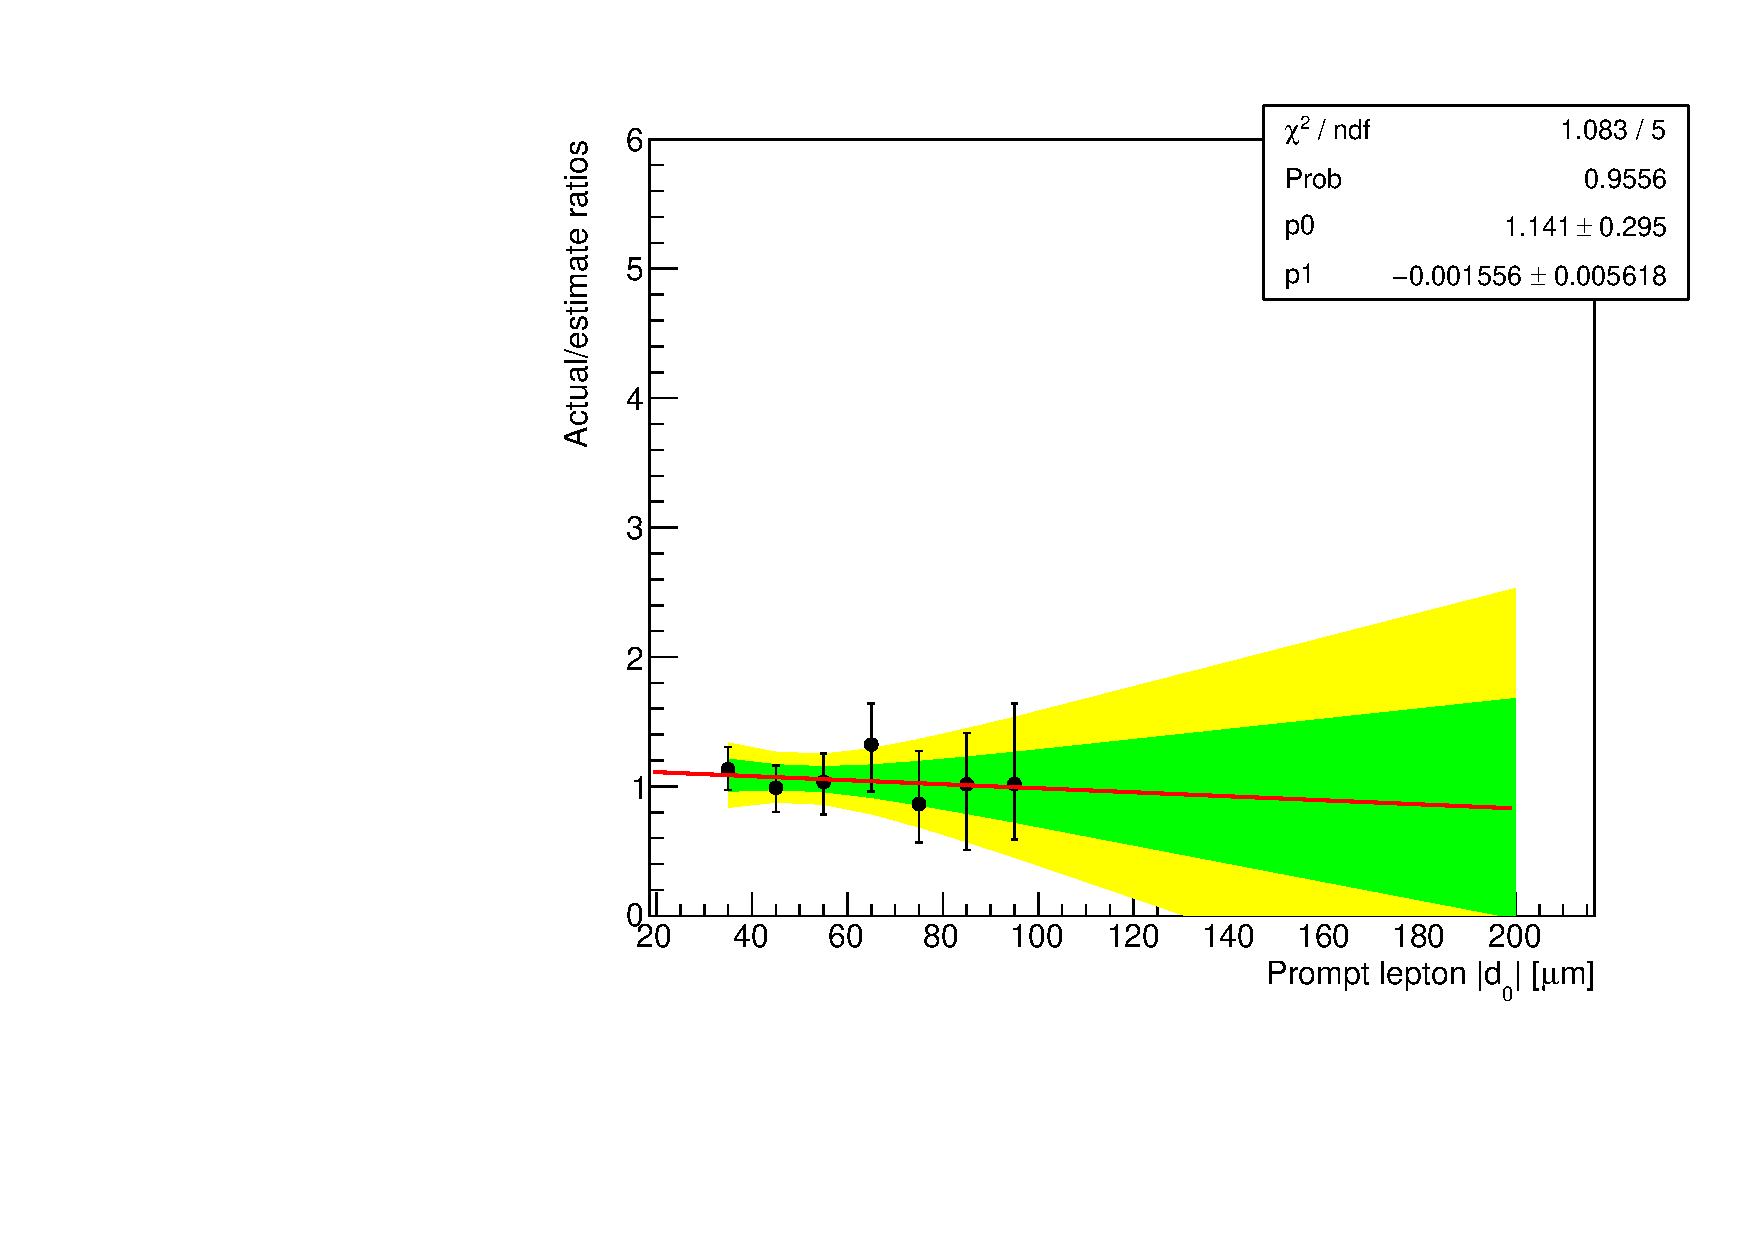
\includegraphics[width=0.45\textwidth]{figures/bg/ee_data_2016_displacedSubleading_ratiosVsPromptD0.pdf}
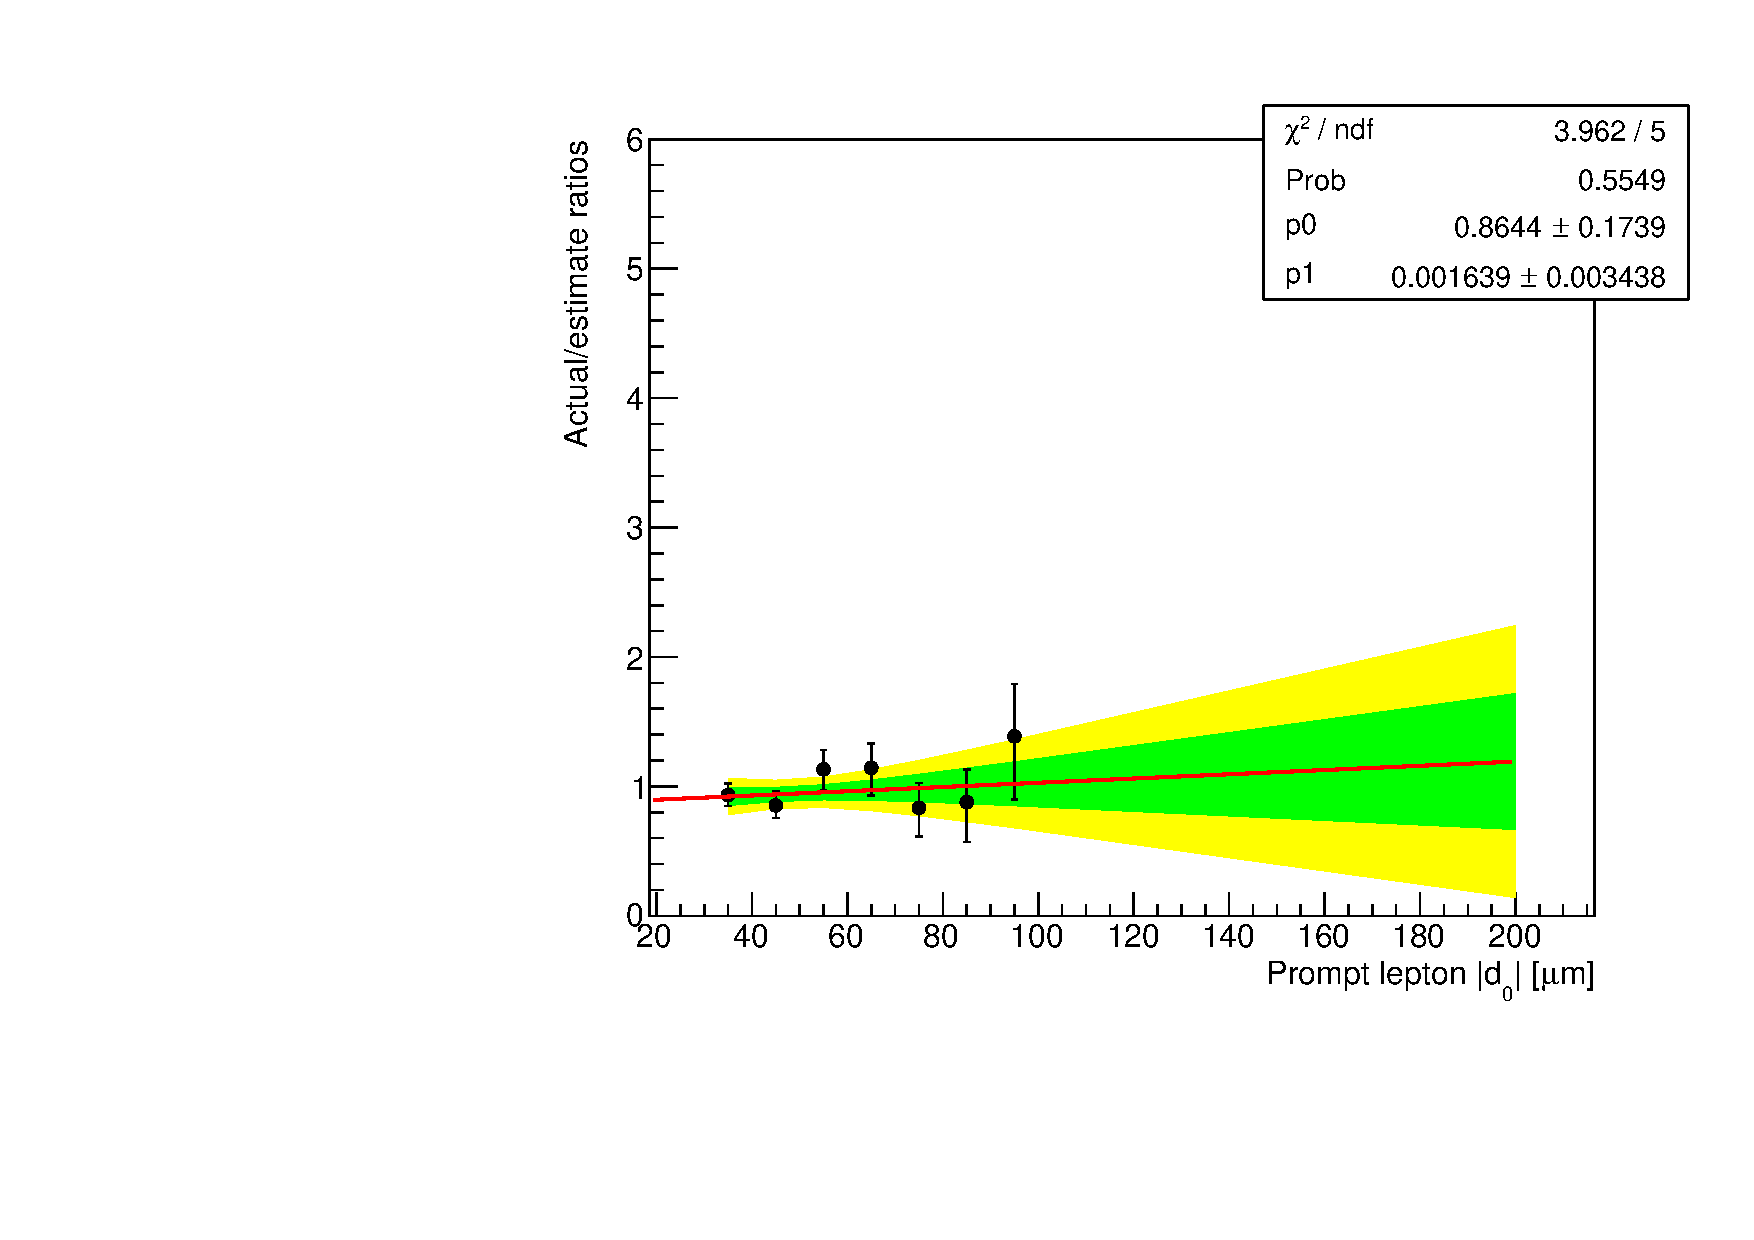
\includegraphics[width=0.45\textwidth]{figures/bg/ee_data_2017_2018_displacedLeading_ratiosVsPromptD0.pdf}
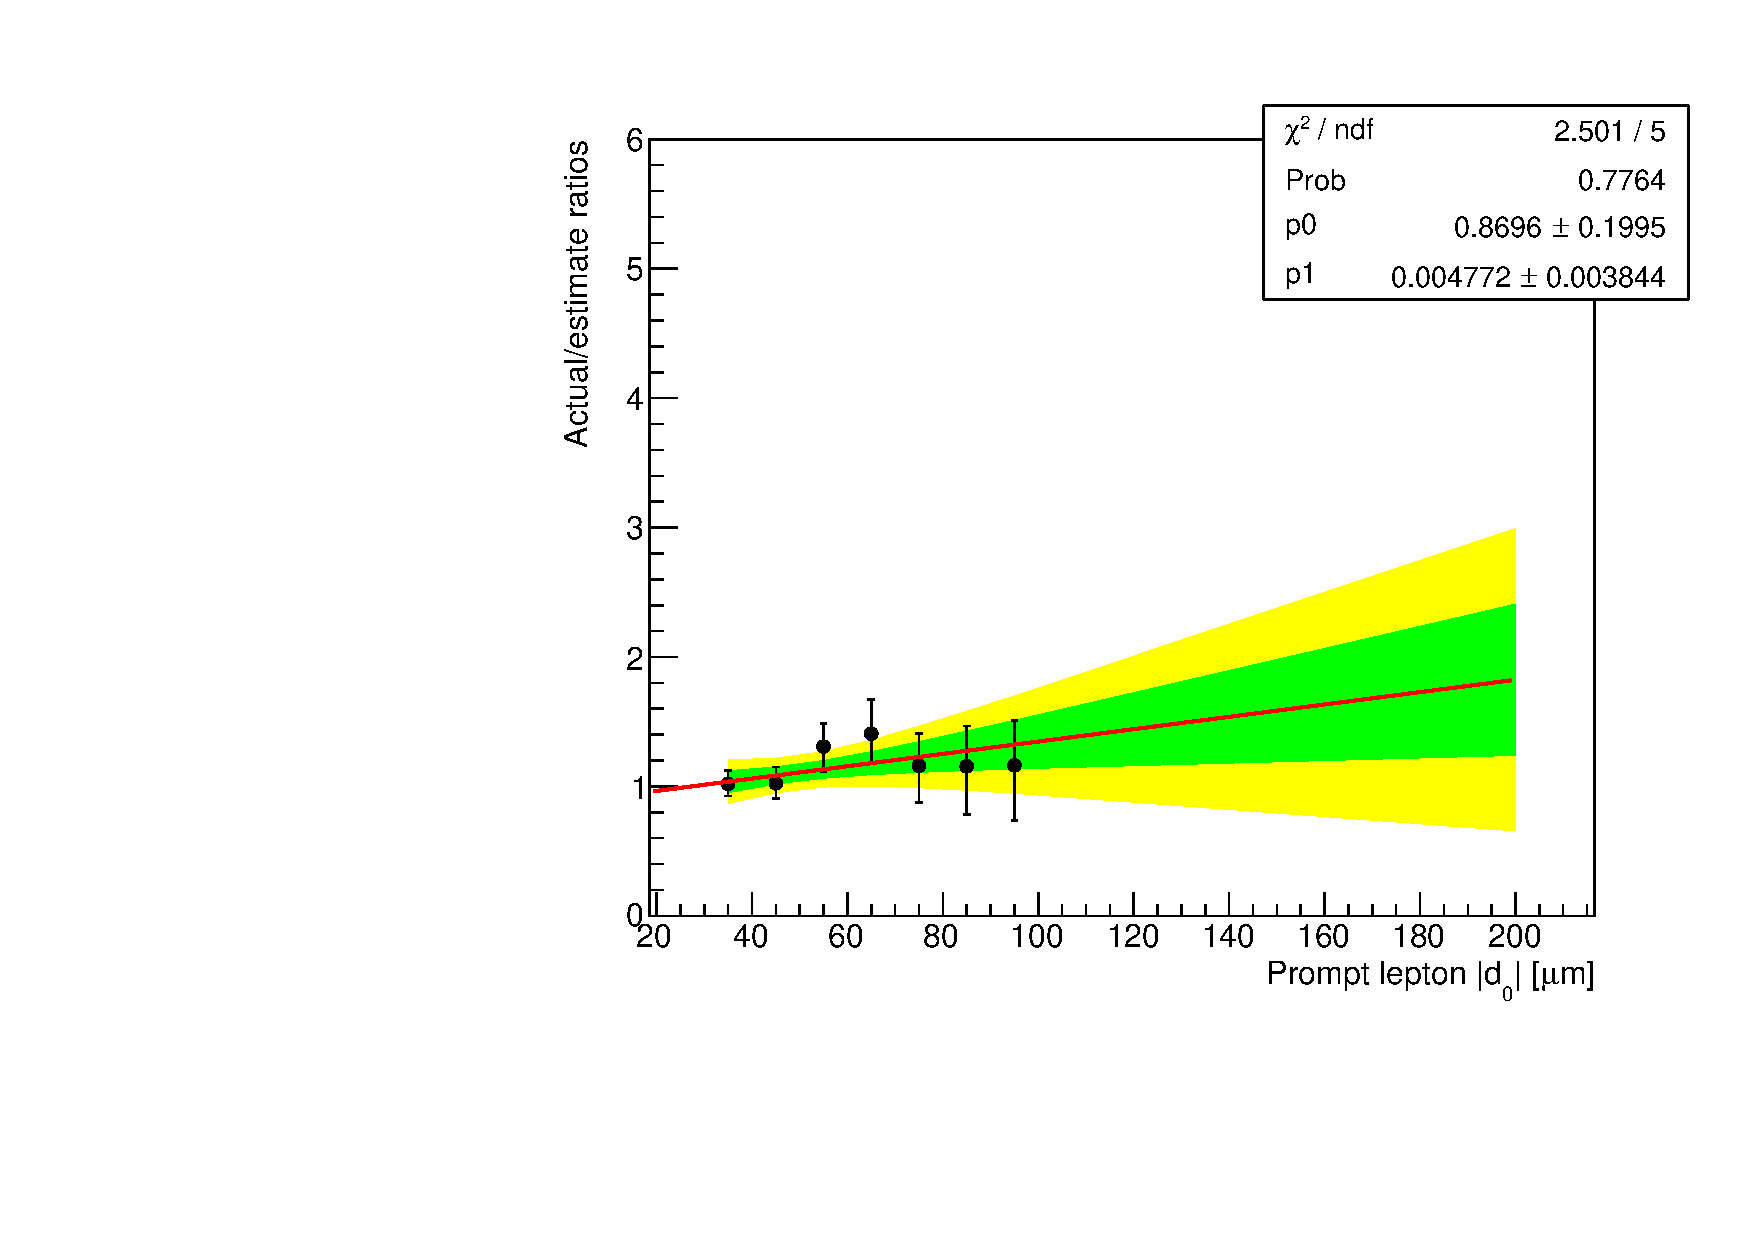
\includegraphics[width=0.45\textwidth]{figures/bg/ee_data_2017_2018_displacedSubleading_ratiosVsPromptD0.pdf}
\caption{Background estimation closure tests in data, in 100--\SI{500}{\um} subregions of regions B (left) and C (right) in the $\Pe\Pe$ channel. Each plot shows the ratio of the actual to the estimated number of events as a function of the prompt lepton \ad in 2016 (top) and 2017--18 (bottom). A linear fit is shown in black along with the \SI{68}{\percent} and \SI{95}{\percent} confidence intervals of the extrapolated fit value.}
\label{100to500um_fits_ee}
\end{figure}


\begin{figure}
\centering
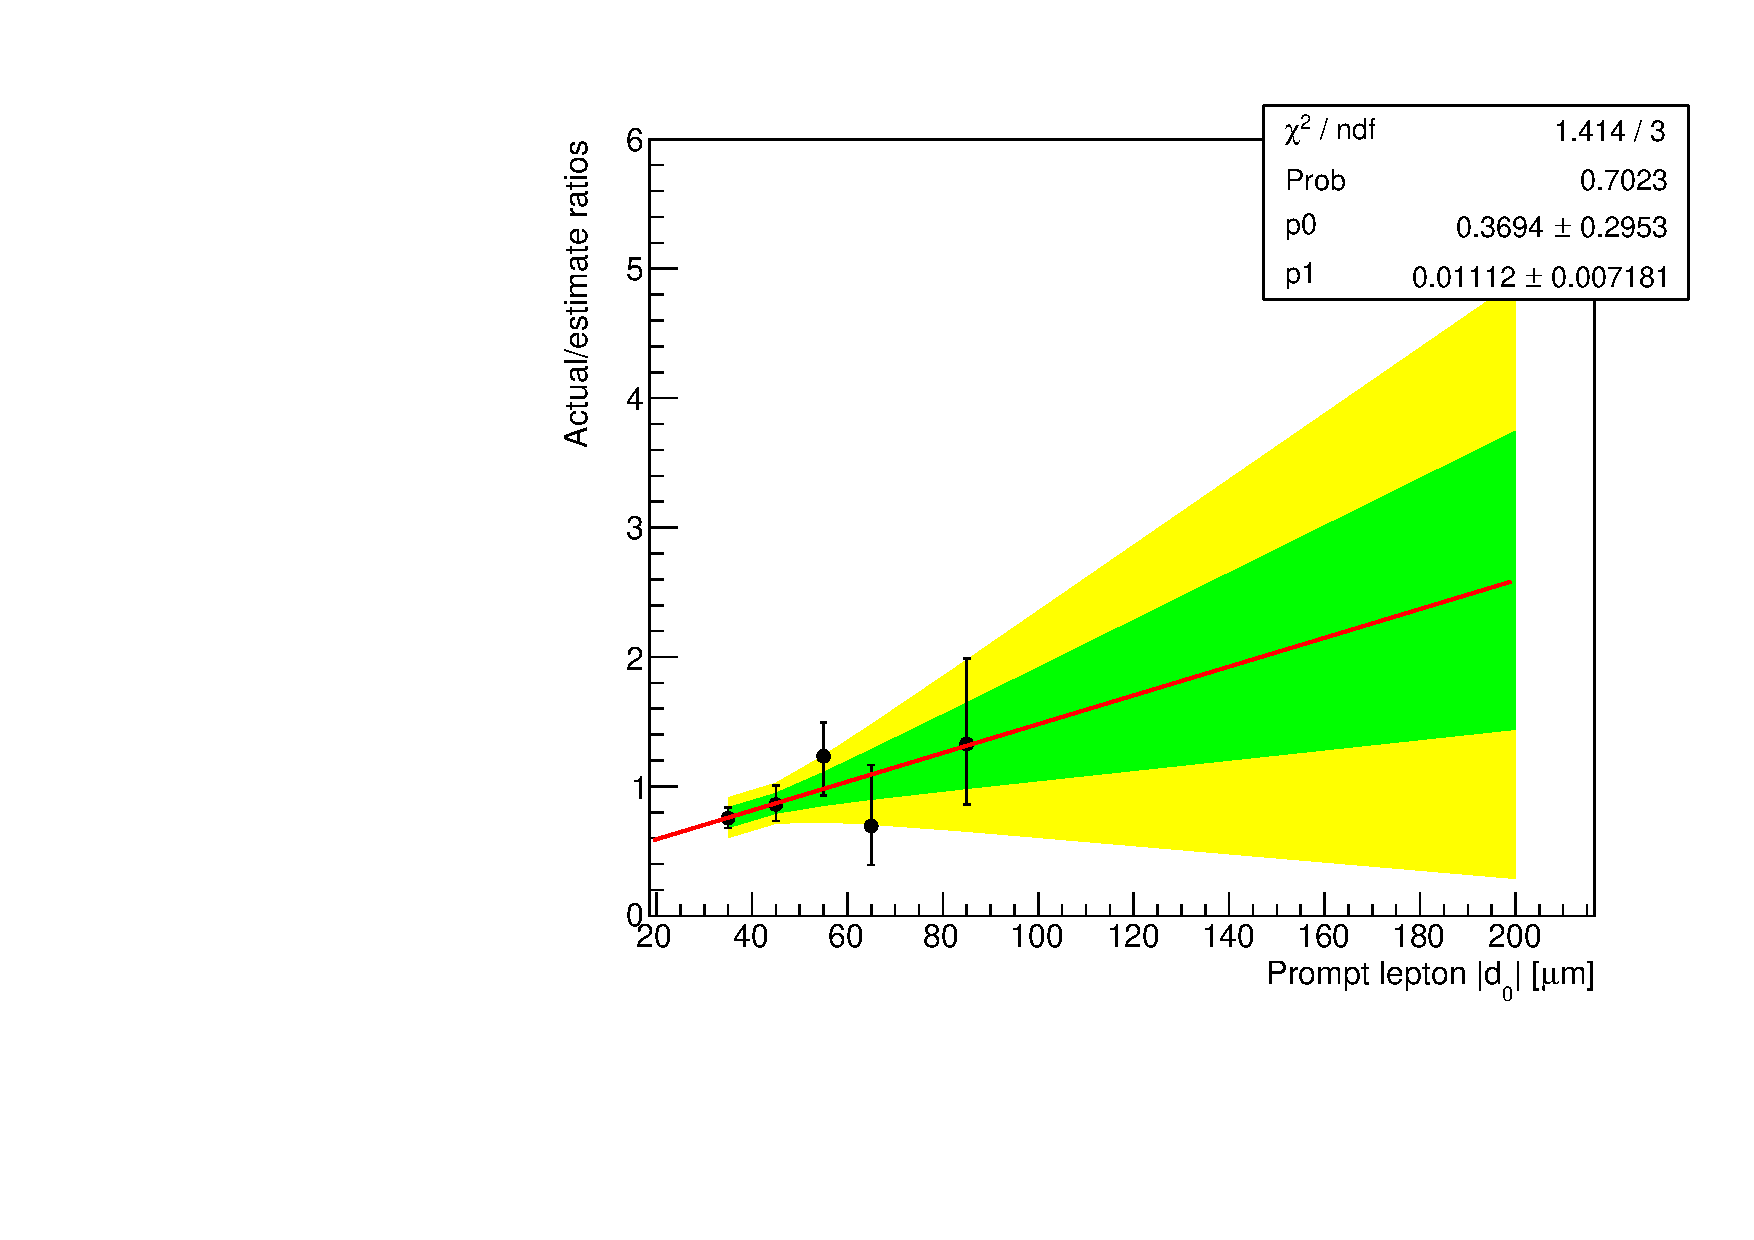
\includegraphics[width=0.45\textwidth]{figures/bg/mumu_data_2016_displacedLeading_ratiosVsPromptD0.pdf}
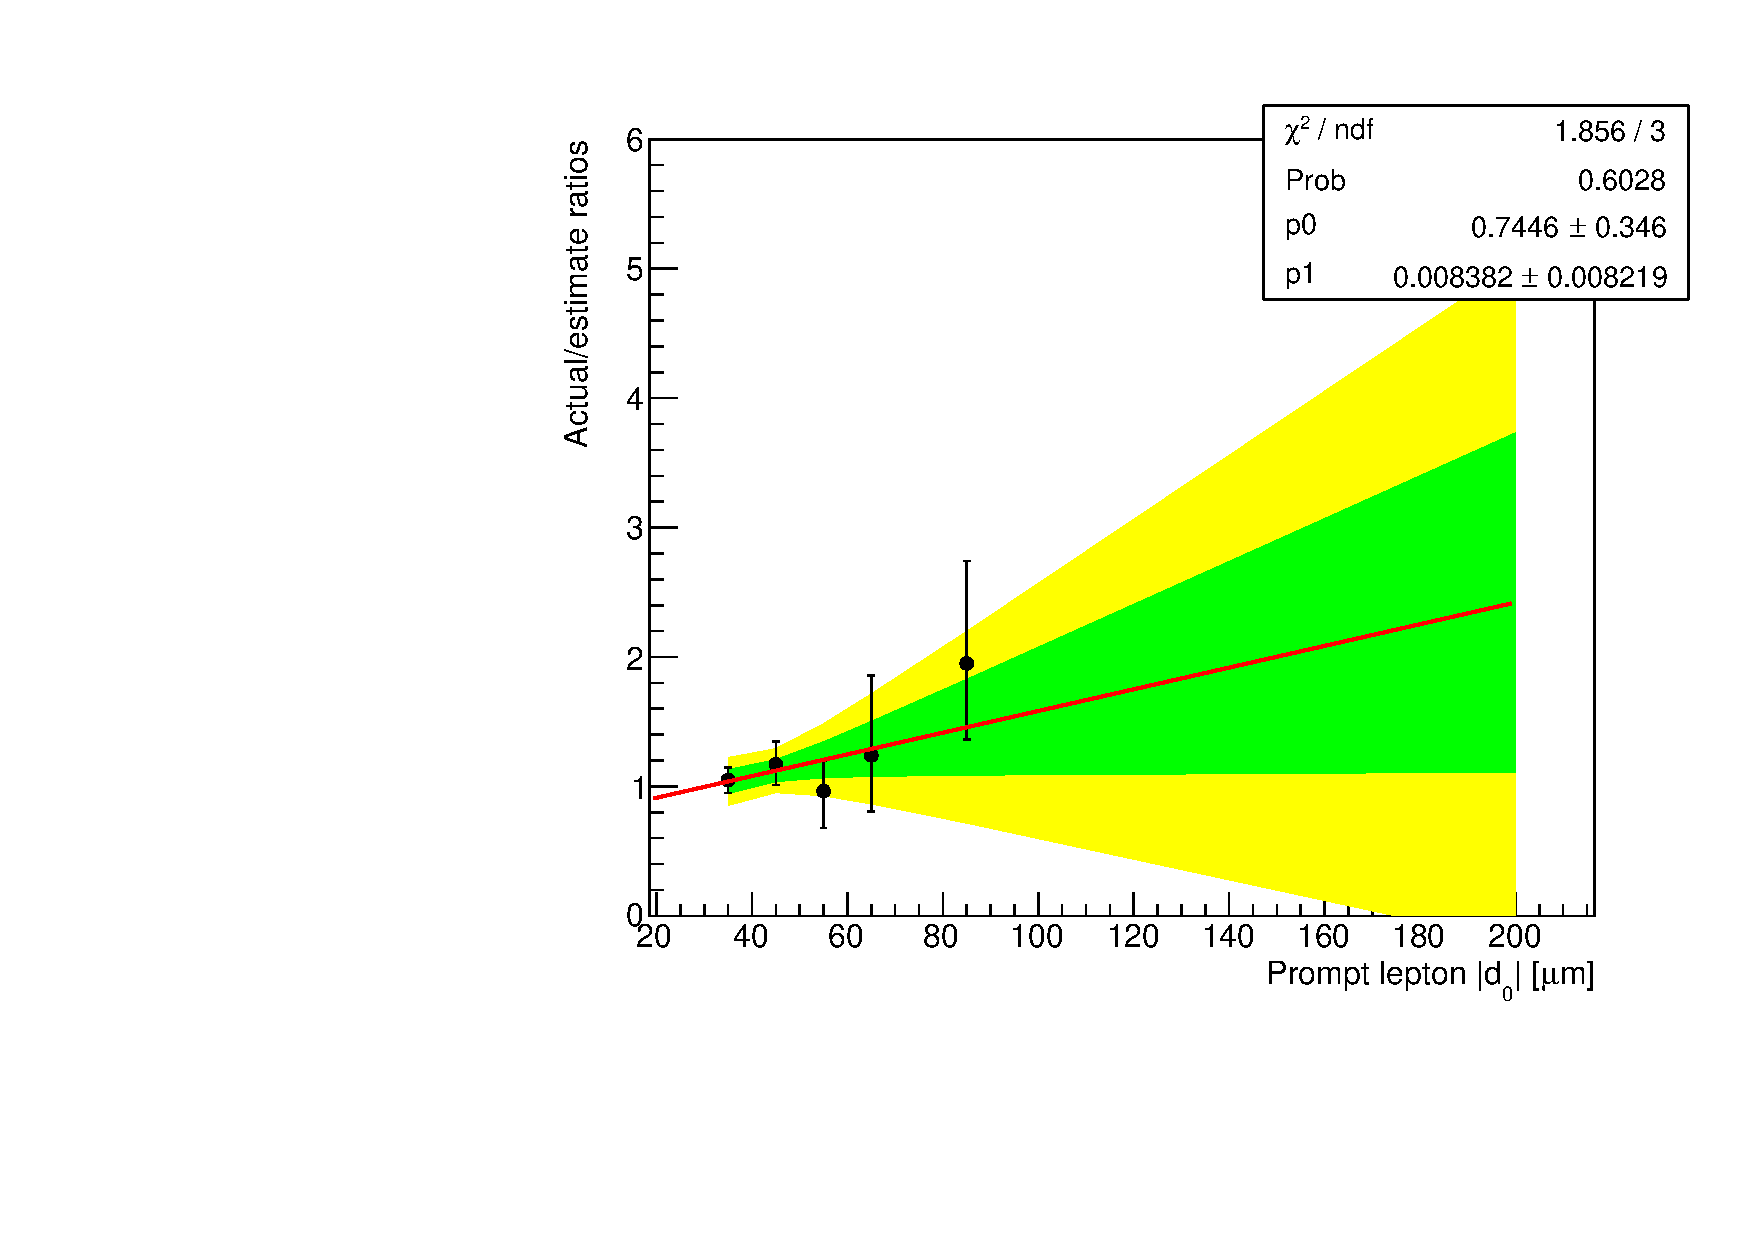
\includegraphics[width=0.45\textwidth]{figures/bg/mumu_data_2016_displacedSubleading_ratiosVsPromptD0.pdf}
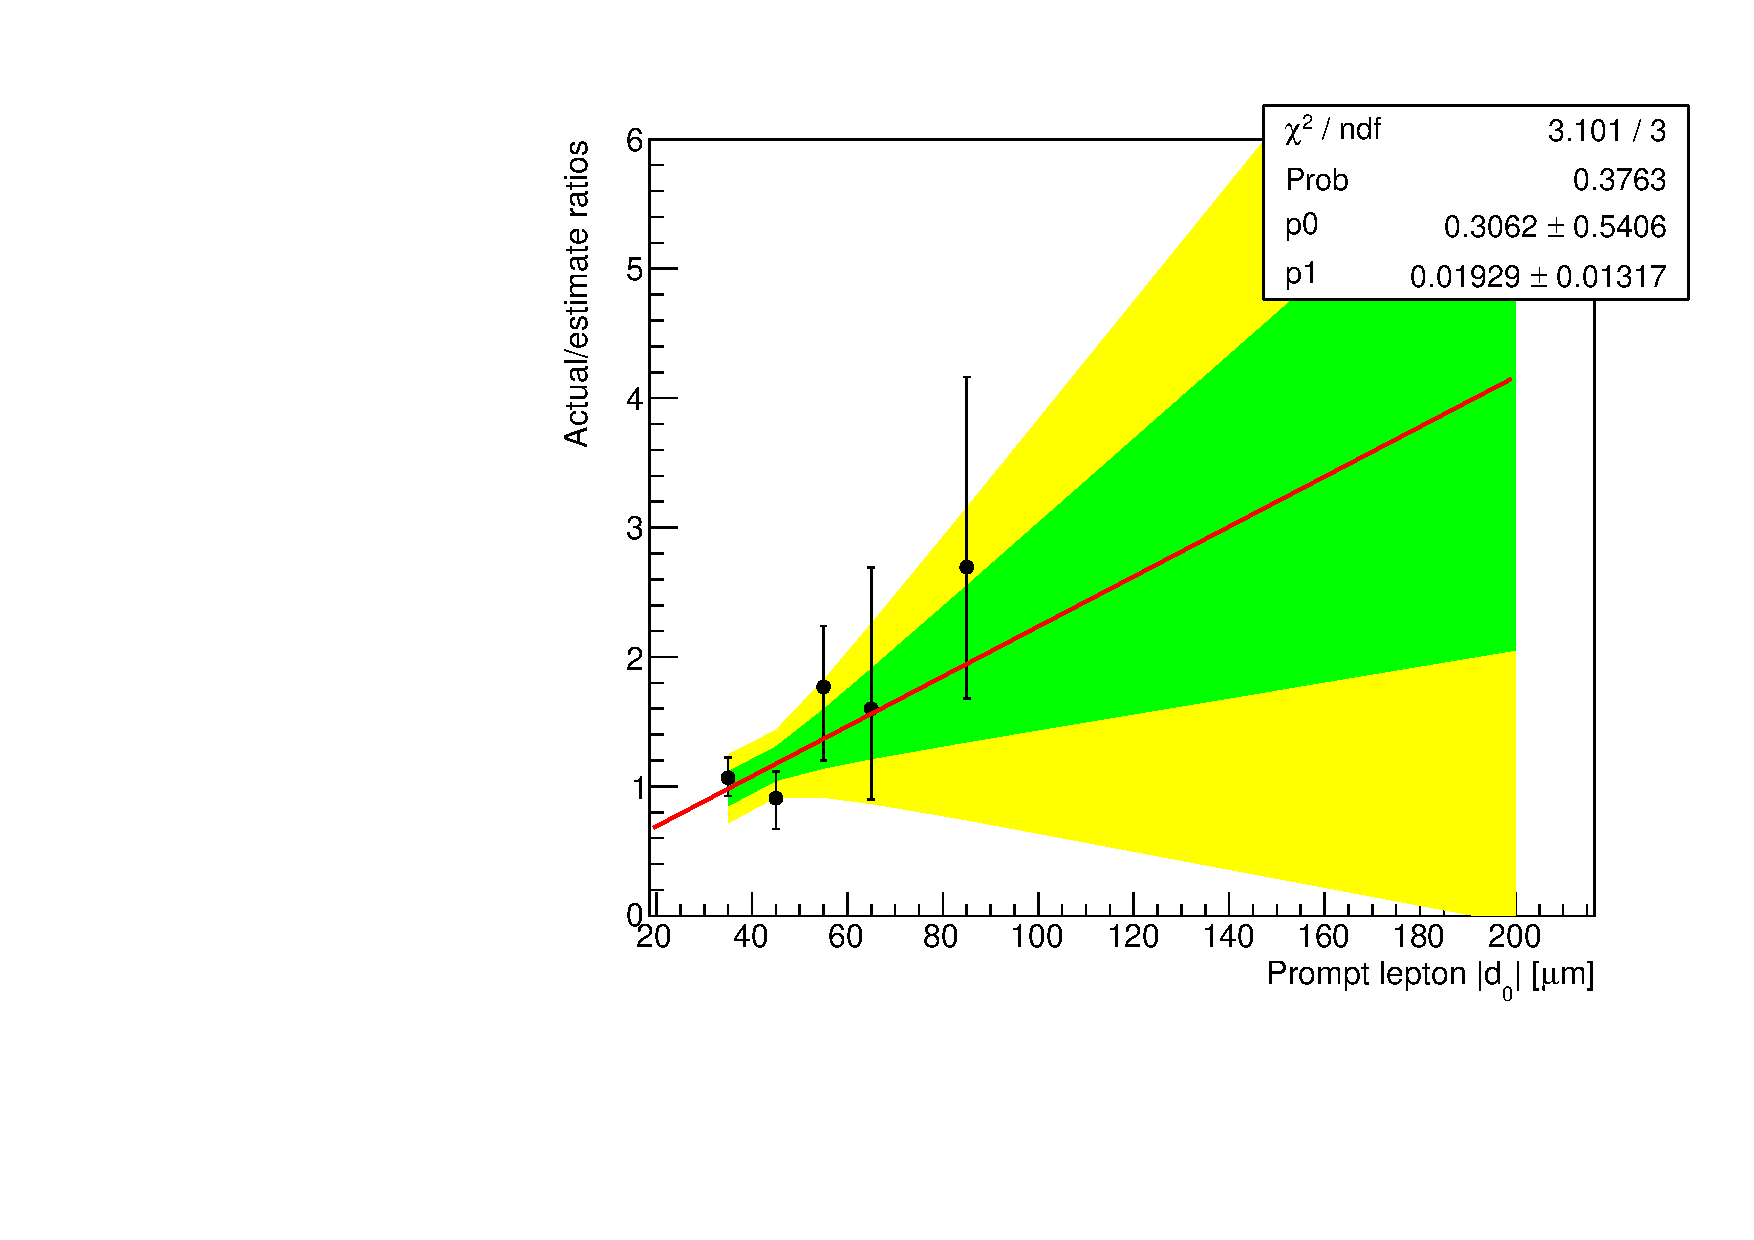
\includegraphics[width=0.45\textwidth]{figures/bg/mumu_data_2017_2018_displacedLeading_ratiosVsPromptD0.pdf}
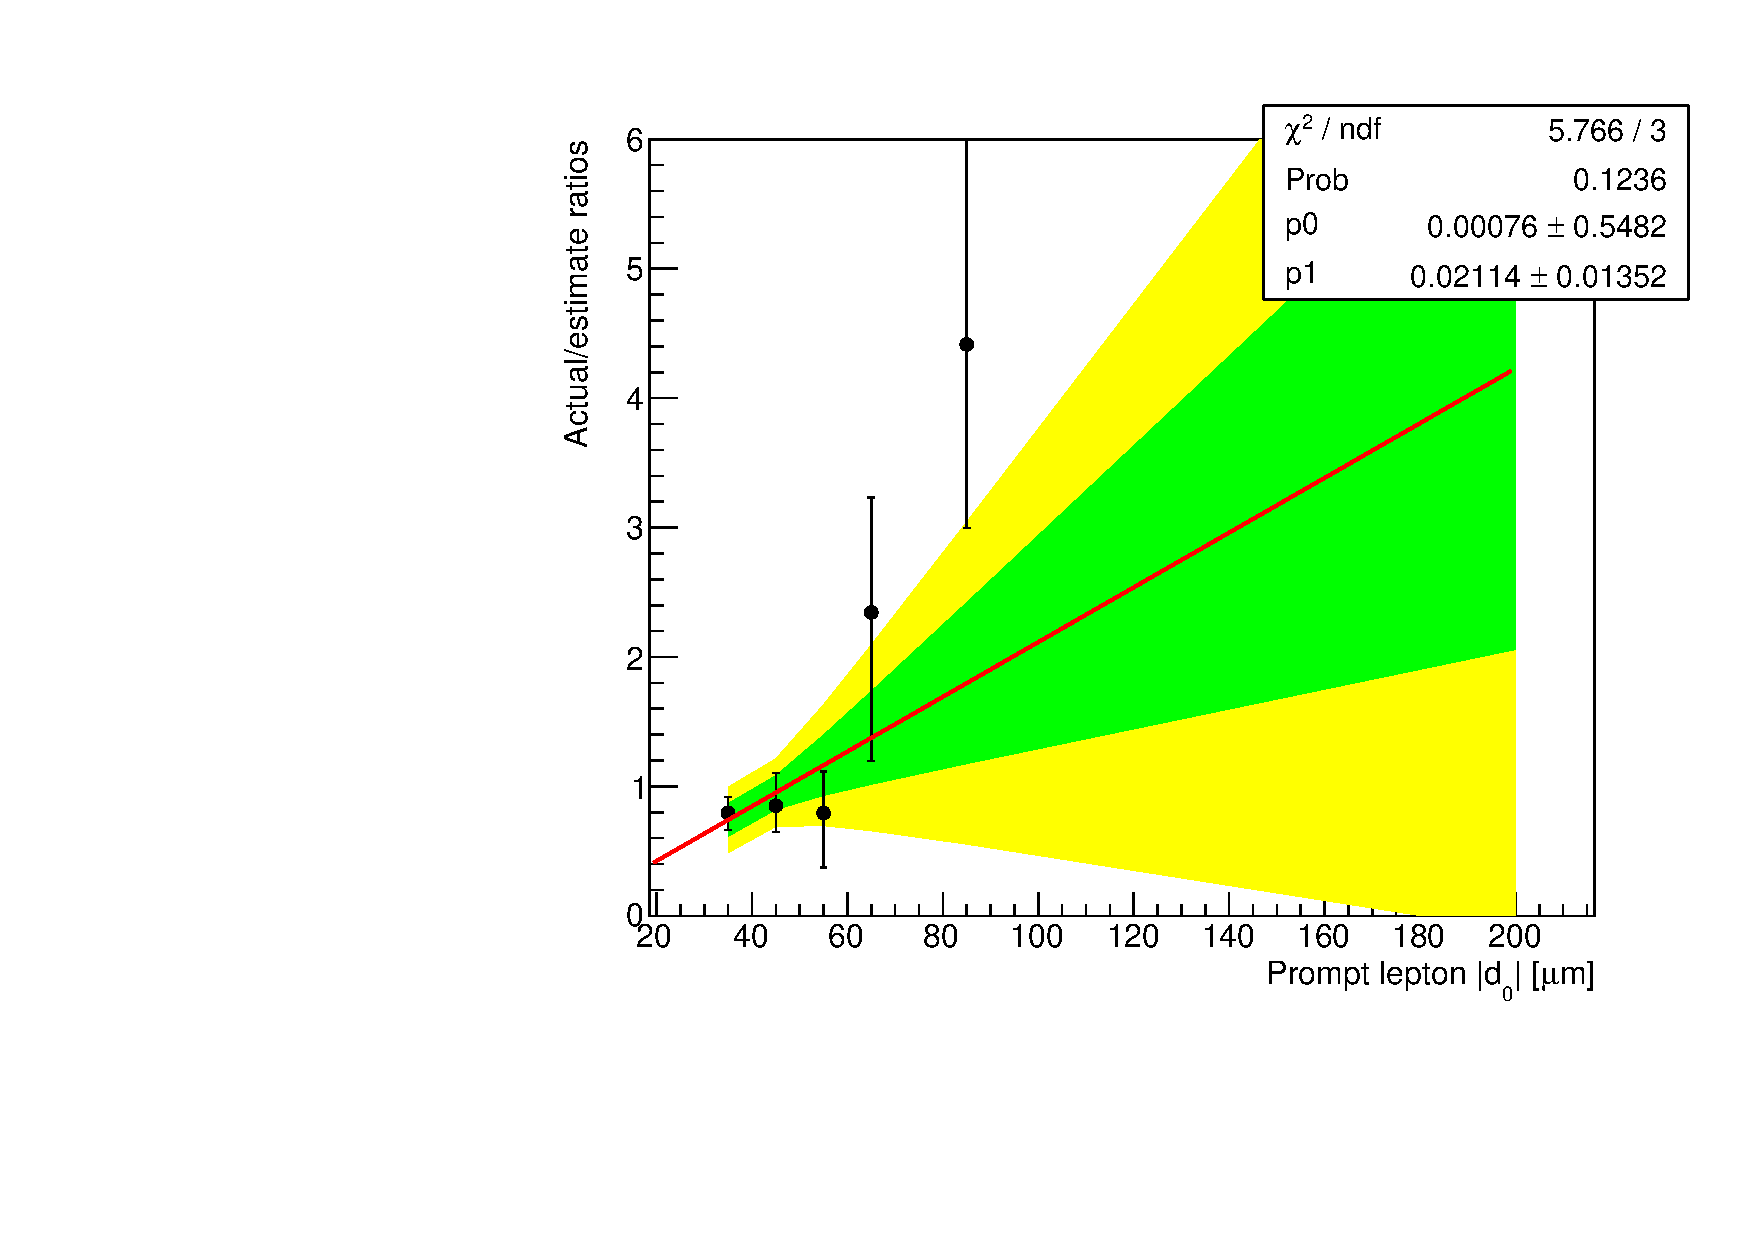
\includegraphics[width=0.45\textwidth]{figures/bg/mumu_data_2017_2018_displacedSubleading_ratiosVsPromptD0.pdf}
\caption{Background estimation closure tests in data, in 100--\SI{500}{\um} subregions of regions B (left) and C (right) in the $\Pgm\Pgm$ channel. Each plot shows the ratio of the actual to the estimated number of events as a function of the prompt lepton \ad in 2016 (top) and 2017--18 (bottom). A linear fit is shown in black along with the \SI{68}{\percent} and \SI{95}{\percent} confidence intervals of the extrapolated fit value.}
\label{100to500um_fits_mumu}
\end{figure}